\subsubsection{802.11}
% 
When wireless networks first came around, it was expected that the radio medium will only be another physical layer, such as cables. However, it did not take long to see that due to significant differences of radio communication, more detailed, radio-suited standard needs to be developed. In 1991 work has begun in preparation of standard that is today known as \emph{802.11} \cite{Hiertz2010TheUniverse}. The scope of this standard is \textquote[\cite{2016IEEEAccess.}]{\emph{to define one medium access control (MAC) and several physical layer (PHY) specifications for wireless connectivity for fixed, portable, and moving stations within a local area.}}\par
One of the most well-known implementations of 802.11 is Wi-Fi. Naturally, it is not the only one and over the years, several amendments have been accepted to initial standard, to accommodate various needs. As Bilgin\&Gungor \cite{Bilgin2013PerformanceAreas} suggest, amendment 802.11b may be used in vehicular environment. Furthermore (and more importantly), amendment 802.11p has been published in 2010. This amendment is designed for the use in transportation, where communication window between two entities may only exist for very limited amount of time and thus some authentication procedures need to be omitted. We will discuss both amendments in following sections.
% 
% 
% 
\subsubsection{802.11b} \label{802.11b}
% 
The 802.11b uses the 2.4GHz unlicensed spectrum and provided increased maximum data rate of 11 Mb/s. It  modulates the data with spread spectrum modulation technique \emph{Direct-sequence spread spectrum} (DSSS). The spread spectrum modulation modifies the signal in a way, that broader spectrum is used than necessarily needed before modulation. Since the signal is spread over more frequencies, it is less vulnerable to interference \cite{MaximIntegratedProductsInc.2013AnMaxim}. The DSSS modulates the signal by multiplying it by pseudo-random  noise-like code (PN) (these are often referred to as chips). The frequency of this code is much higher than the original signal. From Fourier transforms we know that the spectrum of multiplication of two signals will be a convolution of spectra of these signals. Combining wide-band signal (PN) and the narrow band signal (input signal) will result in spectrum that is very similar to the wide-band PN spectrum \cite{Haykin2001CommunicationSystems}. Therefore the output signal is less vulnerable towards narrow-band interference (which may naturally occur in the unlicensed 2.4GHz spectrum).\par
% 
Unlike the original 802.11, which used differential binary phase shift keying (DBPSK) and differential quadrature phase shift keying (DQPSK), the 802.11b uses different type of base-band modulation: \emph{Complementary code keying} (CCK) \cite{2016IEEEAccess.} \cite{Aboul-Magd2008WirelessPerspective}.
CCK is slightly more advanced than orinigal DSSS. Its code words are partially derived from data and static repeating code words are not used. This allows for higher data throughputs in 802.11b \cite{Gast2002802.11Guide}.\par
% 
When we analyse the MAC of 802.11b, we see that it does not differ from the original 802.11 \cite{Gast2002802.11Guide}. Both use the \emph{Distributed coordination function} (DCF) \cite{Hiertz2010TheUniverse}. DCF is a protocol that utilises \emph{Carrier-sense multiple access with collision avoidance} (CSMA/CA) together with binary exponential back-off algorithm. The CSMA/CA listens for broadcast on a channel for a period of time equal to distributed interframe space (DIFS). To understand what DIFS is, we need to explain the Short Interframe Space (SIFS) and Slot time. SIFS is the time wireless interface takes to process a frame (this includes the MAC processing delay and other delays) \cite{2016IEEEAccess.}. Slot time is a value defined for each PHY in the standard \cite{2016IEEEAccess.}. Examples of different values of SIFS and Slot time can be seen in \ref{fig:table-st}. DIFS calculated as \(DIFS = SIFS + ( 2 * Slot time)\). If there is no traffic for period of time equal or greater than DIFS (of the channel is free) only then a frame is transmitted.\par
% 
If during listening period there is traffic (and station received a full frame), then station waits for period of DIFS. If the last frame received by station was not complete/was corrupted, then station waits for Extended interframe spacing (EIFS) (EIFS is longer than SIFS and DIFS). After waiting for this period, the station enters a back-off stage for a random time between 0 and 'connection window' CW. The range of values for CW are specified by \cite{2016IEEEAccess.}. Every time the transmission is not successful, CW is doubled until maximum value is reached. If maximum value is reached, CW is not increased, but the transmission has failed. Successfully transmitted frame is indicated by reception of 'ack frame' (acknowledgement frame). The operation of CSMA/CA can be seen in detail in figure \ref{fig:csma-ca}.\par
% 
% 
\begin{figure}[h]
    \centering
    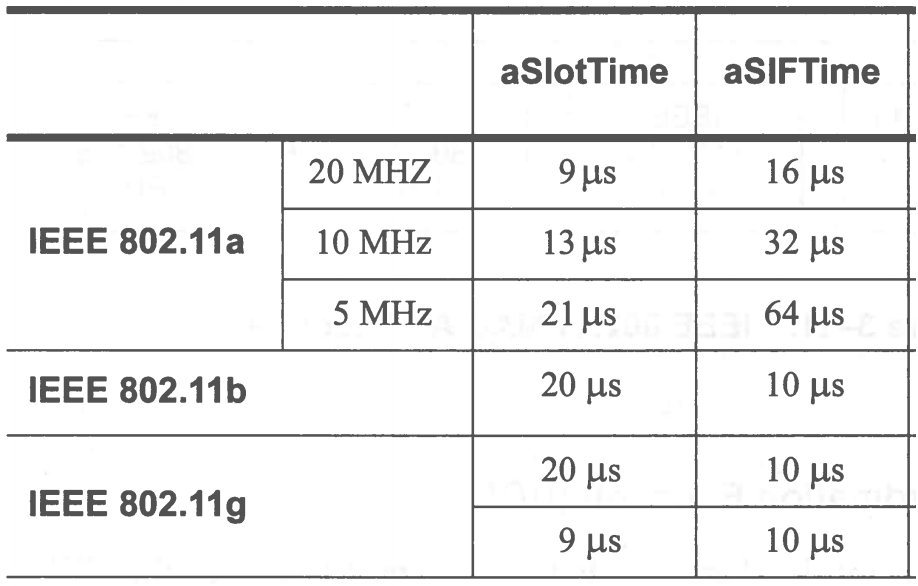
\includegraphics[width=14cm]{table-slot-time}
    \caption{Table showing different values of SIFS and Slot time for different PHY. Taken from \cite{Aboul-Magd2008WirelessPerspective}}
    \label{fig:table-st}
\end{figure}
% 
\begin{figure}
    \centering
    
\includegraphics[height=.95\textheight]{csma-ca}
    \caption{Flowchart showing the operation of CSMA/CA. The dotted square shows RTS/CTS protocol, implementation of which is voluntary. RTS/CTS is part of 802.11 standard. Source: \url{https://commons.wikimedia.org/wiki/File:Csma_ca.svg}}
    \label{fig:csma-ca}
\end{figure}
% 
As for performance of different standards, \cite{Bilgin2013PerformanceAreas} compares 802.11b with 802.11p. The authors compared these in various environments, various speeds and various packet sizes. Since testing this with multiple moving vehicles is very challenging, they used simulation software \emph{MOVE} to generate the movement of vehicles and \emph{NS-2} network simulator to evaluate the parameters of the wireless connection, such as throughput, packet delivery ratio and delay. 
Overall comprehensive analysis provided these results:\\ \textquote[\cite{Bilgin2013PerformanceAreas}]{\emph{Comparative performance evaluations show that IEEE 802.11p MAC layer protocol has better results for V2V communications compared to the IEEE 802.11b MAC protocol in terms of network throughput, end-to-end delay, and delivery ratio.}}\\
This conclusion should not be very surprising, as 802.11p was designed years after 802.11b specifically for use in vehicular environments. We will explore the 802.11p and its uses in the next section.